%!TEX root = Main_Assignment3.tex
\documentclass[Main_Assignment3]{subfiles}

\begin{document}

\section{Specify a software architecture for the Alarm Clock}

The architecture of the system is done with the dividing the system in small component, each testable with either a hardware component or with an interface to these components.
By layering the architecture the it's easier to increase cohesion and reduce the coupling, because the different layers on looks "downwards" and the software components only look at the hardware it is responsible for.
This also creates an abstraction for the higher levels to see functions to handle tasks.

The design will be as in Figure \ref{fig:UML}.
To ensure the components can get the time and the alarm, a singleton is created to encapsulate the methods allowed to be called. 
It will allow \code{get}- and \code{set}-functions for both the alarm and the time. This way all classes have a single way of accessing the classes with anything regarding the time or the alarm.

Since both \code{Alarm} and \code{Clock} has the same key feature - showing a time (be it static or running) they inherit from the interface \code{Time}.

The \code{Controller} is the main loop and will check for all inputs.
It also creates all classes (except for the 2 \code{Time} classes created by the singleton \code{TimeHandler}). 
By doing this \code{Controller} can check whether the alarm should be triggered and activate the \code{Buzzer}, check inputs from \code{Buttons} to whether the current time or alarm should be changed or the projector should be displaying the time.
If \code{Controller} can run a cycle at least every second, the alarm will go off within a second of the actual time.

The patterns to use are polymorphism with the interface and singleton to control the interface.

\begin{figure}[hbtp]
\centering
% 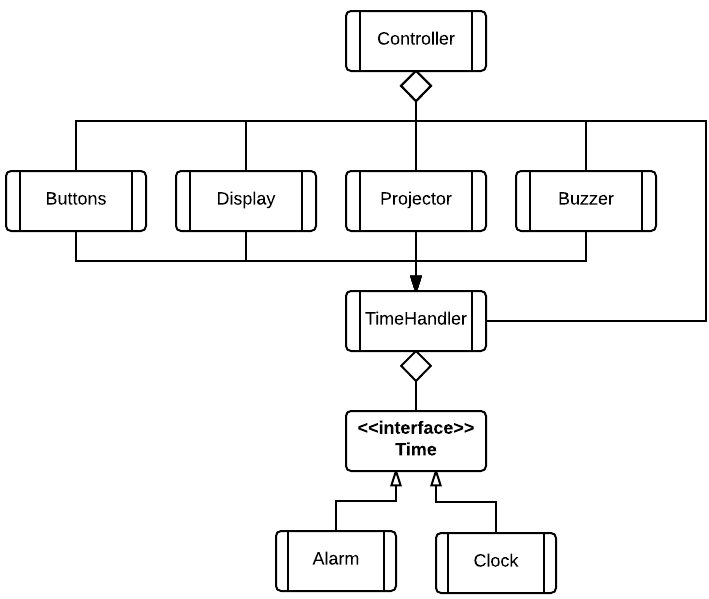
\includegraphics[width = 0.7\textwidth]{ArchitectureDiagram}
\caption{UML diagram}
\label{fig:UML}
\end{figure}

\huge{FIX THIS FIGURE}

\end{document}